\begin{frame}{$SU(N)$ gauge theory}
\begin{figure}
\centering
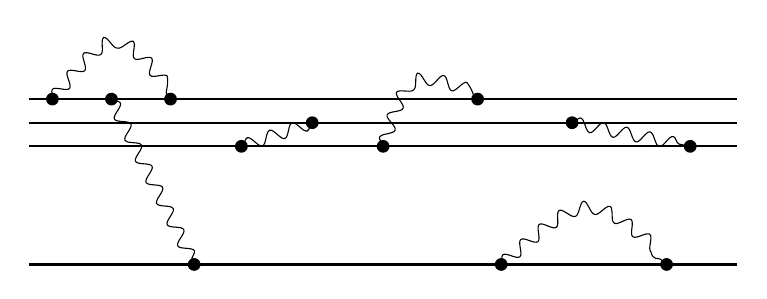
\begin{tikzpicture}[scale=0.3]
% horizontal lines
\draw[ thick] (0,9) -- (30,9);
\draw[ thick] (0,10) -- (30,10);
\draw[ thick] (0,11) -- (30,11);
\draw[ thick] (0,4) -- (30,4);
% strings
\filldraw (1,11) circle [radius=7pt];
\filldraw (6,11) circle [radius=7pt];
\draw[decorate,decoration={snake,amplitude=.8mm,segment length=3mm}] (1,11) .. controls (3.5,14) .. (6,11);
\filldraw (3.5,11) circle [radius=7pt];
\filldraw (7,4) circle [radius=7pt];
\draw[decorate,decoration={snake,amplitude=.8mm,segment length=3mm}] (3.5,11) -- (7,4);

\filldraw (15,9) circle [radius=7pt];
\filldraw (19,11) circle [radius=7pt];
\draw[decorate,decoration={snake,amplitude=.8mm,segment length=3mm}] (15,9) .. controls (16,12) .. (19,11);

\filldraw (23,10) circle [radius=7pt];
\filldraw (28,9) circle [radius=7pt];
\draw[decorate,decoration={snake,amplitude=.8mm,segment length=3mm}] (23,10) -- (28,9);

\filldraw (12,10) circle [radius=7pt];
\filldraw (9,9) circle [radius=7pt];
\draw[decorate,decoration={snake,amplitude=.8mm,segment length=3mm}] (12,10) -- (9,9);

\filldraw (20,4) circle [radius=7pt];
\filldraw (27,4) circle [radius=7pt];
\draw[decorate,decoration={snake,amplitude=.8mm,segment length=3mm}] (20,4) .. controls (23.5,7) .. (27,4);
\end{tikzpicture}
\end{figure}
$N$ D7-branes on top of each other give rise to $N^2$ vector states.
\end{frame}